%TCIDATA{LaTeXparent=0 0 sbrc_2013.tex}
%Review Method

\section{Método do Estudo}\label{sec:review_method}

Este artigo apresenta os resultados de um mapeamento sistemático (MS) de estudos. Um MS tem por objetivo classificar informações acerca de uma área de pesquisa de forma ampla e menos minuciosa que a tradicional revisão sistemática de estudos. Uma vez constatada a vasta quantidade de publicações no campo de SOC, escolheu-se esta metodologia para viabilizar a classifica\c c\~{a}o de um número elevado de artigos. A metodologia adotada seguiu as diretrizes propostas em \cite{petersen:sms2008}, cujos passos necess\'{a}rios s\~{a}o descritos no restante desta se\c c\~{a}o.

\subsection{Protocolo do Estudo}

Um mapeamento sistemático de estudos, assim como outras revisões literárias, estabelece o uso de um protocolo que documenta as etapas do mapeamento de modo a garantir sua replicação e diminuir possíveis erros por parte dos pesquisadores. Nele estão definidas as questões de pesquisa, os fóruns científicos onde as publicações s\~{a}o recuperadas, a \textit{string} de busca utilizada e os critérios de inclusão e exclusão de artigos. 

\subsection{Quest\~{o}es de Pesquisa}\label{sec:questoesPesquisa}

As questões de pesquisa foram organizadas de acordo com a motivação desse estudo, que é investigar e categorizar as contribuições de pesquisa em computação orientada a serviço no contexto de qualidade de serviço. Esse estudo tem como objetivo responder às seguintes perguntas: 

\begin{itemize}
\item {\bf QP1} Qual o interesse de pesquisa da comunidade científica no tema nos \'{u}ltimos anos? 
\item {\bf QP2} Quais áreas de SOC são mais frequentemente pesquisadas no contexto de qualidade de serviços?
\item {\bf QP3} Quais atributos de qualidade são frequentemente considerados nos estudos abordados? 
\item {\bf QP4} Quais s\~{a}o os estudos existentes que mais tem impulsionado QoS em SOC?
\item {\bf QP5} Qual o foco da contribuição de pesquisa realizada?   
\end{itemize}

A QP1 almeja identificar o estado da pesquisa relacionada a SOC no contexto de qualidade de servi\c{c}os em termos quantitativos, ou seja, apontar o n\'{u}mero de contribui\c{c}\~{o}es por ano. A QP2 tem como objetivo trazer uma perspectiva do cen\'{a}rio das pesquisas em Computa\c{c}\~{a}o Orientada a Servi\c{c}o com foco em QoS atualmente. Para responder a essa pergunta, primeiramente definimos quais s\~{a}o as \'{a}reas que melhor caracterizam as diversas contribui\c{c}\~{o}es de pesquisa em SOC. Uma vez definidas essas \'{a}reas, realizamos ent\~{a}o a classifica\c{c}\~{a}o. Com rela\c{c}\~{a}o \`{a} QP3, pretendemos obter com esse estudo quais s\~{a}o os atributos de QoS mais frequentemente explorados em SOC. Em outras palavras, considerando que QoS, nesse contexto, envolve atributos como disponbilidade, confiabilidade, desempenho, seguran\c{c}a, escalabilidade, custo e SLA, quais desses atributos est\~{a}o de fato em foco. Com rela\c{c}\~{a}o \`{a} QP4, pretendemos tamb\'{e}m obter quais s\~{a}o os grupos que mais tem contribu\'{i}do ao contexto desse estudo. Por fim, a QP5 almeja elucidar quais tipos de pesquisa s\~{a}o mais frequentes e inferir conclusões acerca da maturidade da pesquisa realizada na \'{a}rea. Vale ressaltar que no escopo deste artigo n\~{a}o pretendemos avaliar o m\'{e}rito dos trabalhos recuperados.

% 	A QP1 almeja identificar o estado da pesquisa relacionada a SOC no contexto de qualidade de serviços em termos quantitativos, ou seja, apontar o número de publicações na área e os principais autores envolvidos. A QP2 busca mapear quais tópicos receberam maior atenção de pesquisa. Para isso, foram estabelecidas facetas de contribuição capazes de abranger relevantes atividades presentes no campo da computação orientada a serviços. A QP3 visa conhecer quais são, entre os atributos de qualidade de maior notoriedade, os que são com maior frequência contemplados. Além dos atributos de qualidade disponíveis, definiu-se dois outros itens de classificação de contexto. Um para representar a escolha genérica de atributos, isto é, contribuições que não definiram atributos específicos, e outro para representar atributos outros que não estejam definidos como itens de classificação de contexto. 

\subsection{Estratégia de Busca}\label{estrategia_busca}
%Our search strategy consisted of both manual and electronic search. Electronic search was performed in the following digital databases: ACM Digital Library, CiteSeerX, Compendex, Google Scholar, IEEE Xplore and SpringerLink. These are relevant electronic databases to computer science and software engineering, also used in a number of systematic studies in the area [2] .To formulate the search string for electronic database search, we used an approach suggested by Kitchenham [1]. The strategy derives the search string from the research questions using a composition with Boolean operators OR and AND. Table 1 presents the search string. The justification for using manual search was that creativity in RE is a relatively novel area, therefore manual search in conferences and journals provided extra confidence that relevant papers would be found.  To have a more representative set of studies, the “snow-balling" technique was adopted [3], in which the references of the identified papers were analyzed.
Nossa estratégia de busca consistiu essencialmente na busca eletrônica nas seguintes bibliotecas digitais: 
\begin{itemize}
\item ACM Digital Library, 
\item ScienceDirect, 
\item IEEE Xplore, e 
\item SpringerLink.
\end{itemize} 

\noindent Que estão entre as bibliotecas mais relevantes para o contexto da nossa pesquisa. Para formular os termos de busca para a base de dados eletrônica, usamos a abordagem sugerida por Kitchenham~\cite{kitchenham:techReport2007,budgen:ppig2008}. A estrategia 
deriva os termos de busca a partir das questões de pesquisa usando uma composição com os operadores OR e AND. A  Tabela~\ref{tab:exTable1} apresenta a \texttt{string} de busca usada no nosso estudo. Para evitar a tendenciosidade sobre quais comunidades de pesquisa s\~{a}o as mais atuantes no nosso dom\'{i}nio de interesse, assim como obter um tamanho real do volume das contribuições, resolvemos não adotar técnicas como \emph{snow-balling} onde outros trabalhos relacionados podem ser encontrados a partir das referências dos trabalhos extraídos automaticamente \cite{budgen:ppig2008}.

\begin{table}[ht]
\centering
\caption{Termos de Busca utilizados para pesquisa de publicações}
\label{tab:exTable1}
\begin{tabular}{p{0.75\linewidth}}
\hline
((``web service'' OR ``web services'' OR ``service oriented'' OR ``service-oriented'' OR SOA OR SaaS OR PaaS OR ``service orientation'' OR ``service-oriented computing'' OR ``service oriented computing'' OR SOC) AND (``quality of services'' OR ``quality of service'' OR QOS)) \\
\hline
\end{tabular}
\end{table}


\subsection{Crit\'{e}rio de Inclusão e Exclusão}

Para filtrar os artigos coletados, utilizamos os seguintes critérios para inclus\~{a}o e exclus\~{a}o. Inclu\'{i}mos apenas artigos publicados em workshops, confer\^{e}ncias e peri\'{o}dicos nas bibliotecas digitais que satisfaziam nossa \texttt{string} de busca, conforme descrito na Se\c{c}\~{a}o \ref{estrategia_busca}. Artigos considerados como \emph{grey literature}, i.e. relat\'{o}rios t\'{e}cnicos e \emph{white papers}, foram exclu\'{i}dos. No que tange \`{a}s contribui\c{c}\~{o}es em SOC, foram consideradas somente aquelas que lidavam com n\'{i}veis de abstra\c{c}\~{a}o acima do sistema operacional, e.g. relativas a middleware ou plataformas de distribui\c{c}\~{a}o. Contribui\c{c}\~{o}es que lidavam com SOC, mas que n\~{a}o lidavam com nenhum aspecto de QoS foram exclu\'{i}das. Tamb\'{e}m foram exclu\'{i}dos artigos que poderiam ser considerados como resumos estendidos, em geral, aqueles com n\'{u}mero de p\'{a}ginas igual ou inferior a cinco. 

Por fim, para se ter uma perspectiva mais recente do panorama atual, e para tornar o estudo vi\'{a}vel em virtude do volume de publica\c{c}\~{o}es, avaliamos os artigos publicados a partir de 2009 at\'{e} a data da extra\c{c}\~{a}o. O ano foi escolhido com base no hist\'{o}rico num\'{e}rico de publica\c{c}\~{a}o nos \'{u}ltimos cinco anos, conforme gr\'{a}fico de barras da  Figura~\ref{fig:barplotAnoPublicacoes}. Percebemos que houve um \'{a}pice no ano de 2010. Com base nisso, resolvemos fazer uma avalia\c{c}\~{a}o que compreendesse um per\'{i}odo representativo para o mapeamento. Importante destacar que n\~{a}o consideramos o ano de 2012, pois 
nossa a coleta dos artigos compreendeu artigos publicados at\'{e} dezembro 2011.

\begin{figure}[htb]
\centering
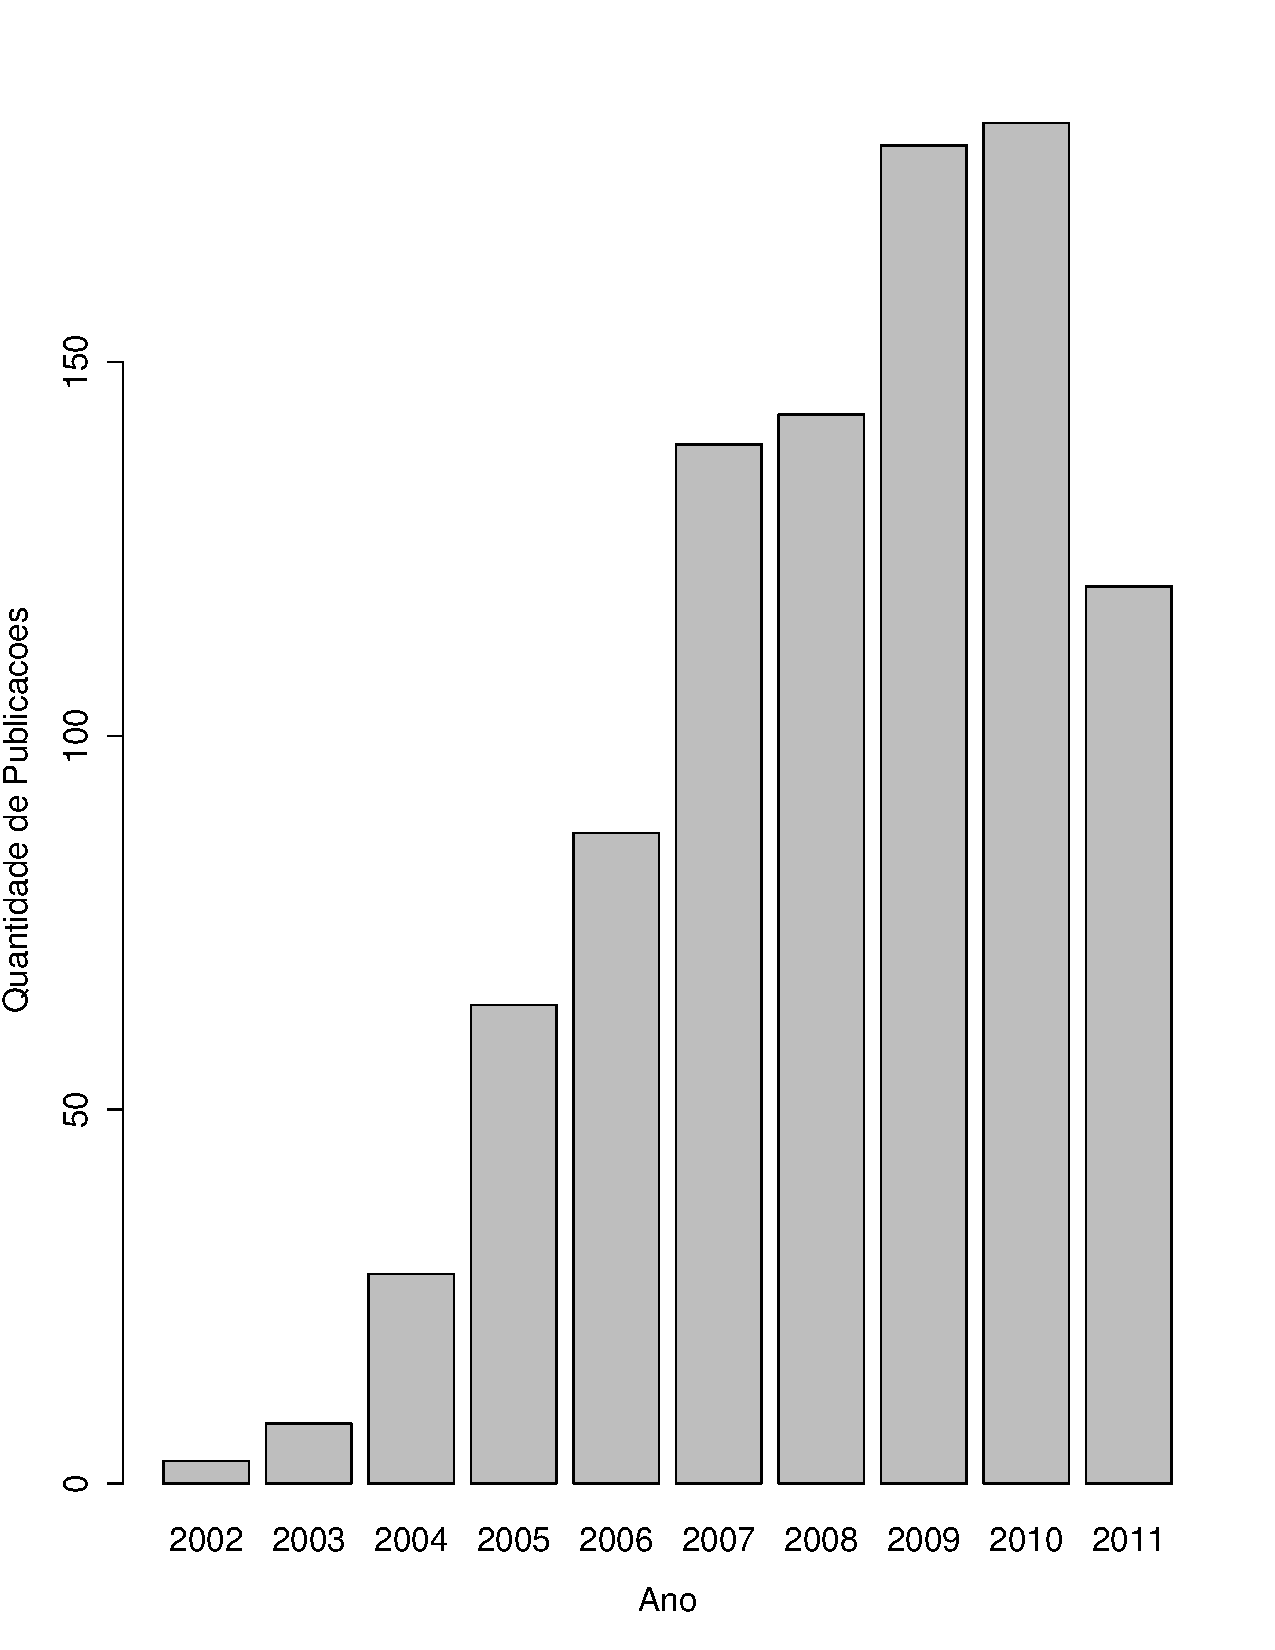
\includegraphics[scale=0.5]{imagens/barplotAnoQuantidadePublicacoes.pdf}
\caption{Quantidade de publica\c c\~{o}es relacionadas a QoS em SOC}
\label{fig:barplotAnoPublicacoes}
\end{figure}

\subsection{Coleta, Armazenamento dos Dados e Análise}

Inicialmente foram feitas consultas manuais em cada uma das bibliotecas digitais mencionadas na Se\c c\~{a}o~\ref{estrategia_busca}. Verificou-se ao todo um número de 1034 publicações a serem analisadas. Para atender a essa quantidade significativa de publica\c c\~{o}es, a coleta dos resultados de busca foi automatizada por um \emph{crawler} capaz de recuperar as publica\c c\~{o}es nas bibliotecas digitais e armazenar as mesmas 
em banco de dados local. Mais especificamente, o \emph{crawler} armazena os metadados das publicações resultantes das buscas nas diferentes bibliotecas.

%Descrever como o ambiente no Heroku está organizado (facets), explicar os termos principalmente os de Computação Orientada a Serviços qual a referência de significado que usamos. ``Each author individually extracted data from a subset of papers. We jointly  discussed unclear issues and solved discrepancies in the analysis.'' Os resultados tambem foram gerados automaticamente por meio da propria ferramenta....

Com base na experi\^{e}ncia de alguns dos autores deste artigo, que tinham observado a dificuldade em se trabalhar com revis\~{o}es sistem\'{a}ticas de forma cooperativa utilizando planilhas eletr\^{o}nicas, decidimos desenvolver uma ferramenta de apoio para permitir a an\'{a}lise e 
classifica\c c\~{a}o dos artigos com maior eficiência e ubiquidade de trabalho, suportando a gera\c c\~{a}o dos 
resultados sumarizados em gr\'{a}ficos 
em tempo real. Esta ferramenta consiste em um ambiente disponível na nuvem, com interfaces disponíveis para a listagem das publicações coletadas automaticamente pelo \emph{crawler} ou de forma manual pela interface de registro de novas publicações.

No ambiente dessa ferramenta, cada publicação pode ser classificada por meio de uma interface apropriada que contém os metadados do artigo, campos de anotações e marcações dos itens de classificação definidos para o mapeamento de estudos em questão. O uso dessa ferramenta foi de grande importância para a viabilidade do MS diante da quantidade inicial de publicações coletadas. Al\'{e}m disso, tal ferramenta permitiu 
a realiza\c{c}\~{a}o do mapeamento de forma colaborativa onde os artigos s\~{a}o compartilhados entre diferentes grupos de usuários em suas respectivas sess\~{o}es autenticadas.

A partir da distribuição automática de artigos para cada um dos pesquisadores, foram excluídas manualmente as publicações que não se adequaram aos critérios definidos. Tal processo, assim como a classificação, foi realizado individualmente, tendo havido frequente discussão para eliminar quaisquer dúvidas e inconsistências de interpretações quanto aos critérios de inclusão, exclusão e facetas de classificação. 

Os artigos foram classificados de acordo com as categorias:
\begin{itemize}
\item[-] \textbf{Contribuição}: composição, coordenação e comunicação, descoberta e seleção, ciclo de vida, monitoramento e adaptação, modelos de QoS e linguagens. As definições usadas para as facetas de contribuição são definidas conforme~\cite{SCUBE}. Em particular, a categoria \emph{modelos de QoS e linguagens} engloba publicações que definem extensões ou novos modelos de QoS por meio de linguagens, especificações e ontologias a serem utilizadas em sistemas baseados em serviços e na definição de contratos de serviços que incluam garantias de QoS
\item[-] \textbf{Contexto}: disponibilidade, desempenho, confiabilidade, escalabilidade, segurança, SLA, custo, outros)... (EXPLICAR EM PARTICULAR SLA). 
\item[-] \textbf{Pesquisa}: solução, avaliação, validação e experiência pessoal. Em particular, diferenciamos a caracter\'{i}stica \emph{avalia\c{c}\~{a}o} de \emph{valida\c{c}\~{a}o} conforme \cite{Wiering et al. 2006}. Artigos classificados em avalia\c{c}\~{a}o s\~{a}o aqueles que .... Enquanto que os artigos avaliados em valida\c{c}\~{a}o s\~{a}o aqueles que .... No entanto, vale ressaltar que artigos classificados como solu\c{c}\~{a}o podem tamb\'{e}m podem ser mapeados como valida\c{c}\~{a}o ou avalia\c{c}\~{a}o, caso estas fa\c{c}am parte da contribui\c{c}\~{a}o do trabalho estudado.
\end{itemize}

%\begin{itemize}
%\item {\bf Composição} Trata da agregação de serviços visando o estabelecimento de novas aplicações ou seu rearranjo de forma a manter determinados níveis de QoS pré-estabelecidos ou acordados.
%\item {\bf Coordenação e Comunicação} Trata da orquestração de serviços para atender a um objetivo determinado num período de duração correspondente à atividade executada. Além disso, envolve a troca de mensagens através do orquestrador, portanto também envolve protocolos específicos para a transação e comunicação em geral.
%\item {\bf Descoberta e Seleção} Refere-se à publicação, descoberta e seleção de serviços em registros públicos ou privados considerando aspectos de qualidade de serviços.
%\item {\bf Ciclo de vida} Refere-se às fases da engenharia de software dentro do domínio de sistemas baseados em serviços, tal qual projeto, desenvolvimento, manutenção e testes.
%\item {\bf Monitoramento e Adaptação} Relacionados ao tempo de execução, monitoramento de atributos não funcionais e adaptação de configuração e disposição de serviços visando manter os níveis desejados de QoS.
%\item {\bf Modelos de QoS e Linguagens} Engloba publicações que definem extensões ou novos modelos de QoS por meio de linguagens, especificações e ontologias a serem utilizadas em sistemas baseados em serviços e na definição de contratos de serviços que incluam garantias de QoS.
%\end{itemize} 